\documentclass[12pt]{article}
\usepackage{verbatim}
\usepackage[dvips]{epsfig}
\usepackage{color}
\usepackage{url}
\usepackage[colorlinks=true]{hyperref}

\begin{document}

\section*{GENESIS: Documentation}

{\bf Related Documentation:}
% start: userdocs-tag-replace-items related-do-nothing
% end: userdocs-tag-replace-items related-do-nothing

\subsection*{Figure\,13}

\begin{figure}[h]
\centering
   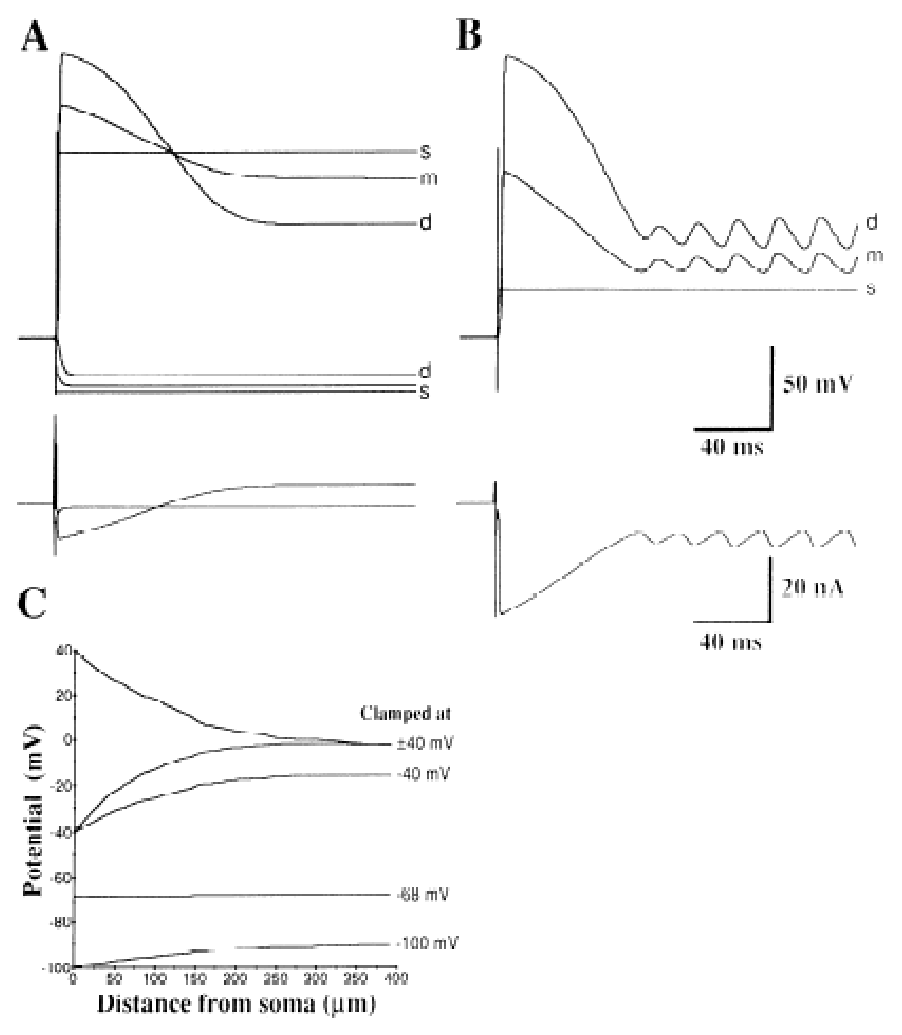
\includegraphics[scale=0.75]{figures/Fig.1.13.eps}
   \caption{Simulation of voltage-clamp steps. $A$: Model was clamped at resting potential (-68\,mV) and then stepped to -100 or +40\,mV. Superimposed top traces: membrane potential in the soma (s), main dendrite (m), and a distal spiny dendrite (d, marked with asterisk in \href{../pub-purkinje-deschutter1-fig-1/pub-purkinje-deschutter1-fig-1.tex}{\bf Fig.\,1}). Bottom trace: clamp current. $B$: as in $A$, but stepped to -40\,mV. $C$: membrane potential under steady-state voltage clamp vs. distance from the soma. Data from the same voltage-clamp steps as shown in $A$ and $B$. Data points are exclusively from compartments linking the soma with the distal spiny dendrite. Because the potential oscillated during steps to -40\,mV, 2 traces are shown for that voltage step (corresponding to the minimum and maximum voltage in the spiny dendrite). Simulation time step was 5\,$\mu$s.}
   \label{fig:DS1.13}
\end{figure}

\bibliographystyle{plain}
\bibliography{../tex/bib/g3-refs.bib}

\end{document}
